\newcommand{\Person}[1]{
\draw[ultra thick] (#1) circle (.4cm);
}
\newcommand{\Exposed}[1]{
\draw[ultra thick,fill=gray!50] (#1) circle (.4cm);
}
\newcommand{\Sick}[1]{
\draw[ultra thick] (#1) -- +(.25,.25);
\draw[ultra thick] (#1) -- +(.25,-.25);
\draw[ultra thick] (#1) -- +(-.25,-.25);
\draw[ultra thick] (#1) -- +(-.25,.25);
}
\newcommand{\PersonSick}[1]{
\Person{#1}
\Sick{#1}
}
\newcommand{\ExposedSick}[1]{
\Exposed{#1}
\Sick{#1}
}

The diagrams below show 4 different diseases --- A, B, C, D --- along with exposure to
some hypothesized cause.  For each of the 4 diseases, say whether the
exposure is necessary and/or sufficient.

Key:
\begin{itemize}
\item Exposed but not sick 
\begin{tikzpicture} \Exposed{0,0} \end{tikzpicture}
\item Sick 
\begin{tikzpicture} \PersonSick{0,0} \end{tikzpicture}
\item Exposed and Sick 
\begin{tikzpicture} \ExposedSick{0,0} \end{tikzpicture}
\item Neither exposed nor sick 
\begin{tikzpicture} \Person{0,0} \end{tikzpicture}
\end{itemize}


\begin{tabular}{||c|||c||}\hline\hline
Disease A %Necessary and Sufficient 
&  
Disease B %Necessary but not Sufficient
\\
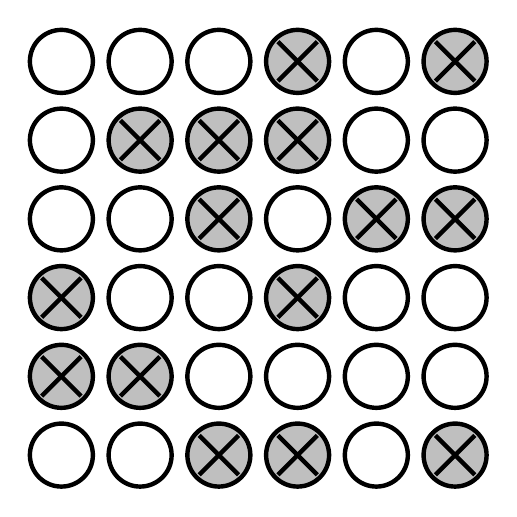
\begin{tikzpicture}
\Person{0,0}\ExposedSick{0,1}\ExposedSick{0,2}\Person{0,3}\Person{0,4}\Person{0,5}
\Person{1,0}\ExposedSick{1,1}\Person{1,2}\Person{1,3}\ExposedSick{1,4}\Person{1,5}
\ExposedSick{2,0}\Person{2,1}\Person{2,2}\ExposedSick{2,3}\ExposedSick{2,4}\Person{2,5}
\ExposedSick{3,0}\Person{3,1}\ExposedSick{3,2}\Person{3,3}\ExposedSick{3,4}\ExposedSick{3,5}
\Person{4,0}\Person{4,1}\Person{4,2}\ExposedSick{4,3}\Person{4,4}\Person{4,5}
\ExposedSick{5,0}\Person{5,1}\Person{5,2}\ExposedSick{5,3}\Person{5,4}\ExposedSick{5,5}
\end{tikzpicture}
&
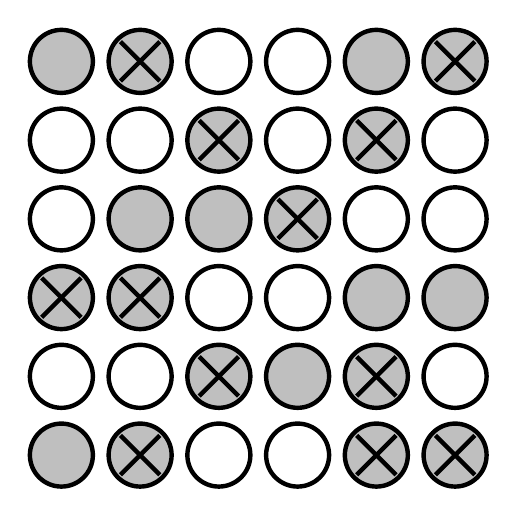
\begin{tikzpicture}
\Exposed{0,0}\Person{0,1}\ExposedSick{0,2}\Person{0,3}\Person{0,4}\Exposed{0,5}
\ExposedSick{1,0}\Person{1,1}\ExposedSick{1,2}\Exposed{1,3}\Person{1,4}\ExposedSick{1,5}
\Person{2,0}\ExposedSick{2,1}\Person{2,2}\Exposed{2,3}\ExposedSick{2,4}\Person{2,5}
\Person{3,0}\Exposed{3,1}\Person{3,2}\ExposedSick{3,3}\Person{3,4}\Person{3,5}
\ExposedSick{4,0}\ExposedSick{4,1}\Exposed{4,2}\Person{4,3}\ExposedSick{4,4}\Exposed{4,5}
\ExposedSick{5,0}\Person{5,1}\Exposed{5,2}\Person{5,3}\Person{5,4}\ExposedSick{5,5}
\end{tikzpicture}
\\\hline\hline
Disease C %Not necessary but Sufficient 
& 
Disease D %Neither Necessary nor Sufficient
\\
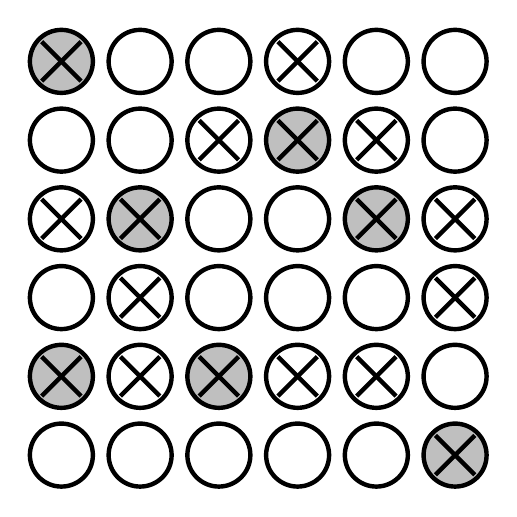
\begin{tikzpicture}
\Person{0,0}\ExposedSick{0,1}\Person{0,2}\PersonSick{0,3}\Person{0,4}\ExposedSick{0,5}
\Person{1,0}\PersonSick{1,1}\PersonSick{1,2}\ExposedSick{1,3}\Person{1,4}\Person{1,5}
\Person{2,0}\ExposedSick{2,1}\Person{2,2}\Person{2,3}\PersonSick{2,4}\Person{2,5}
\Person{3,0}\PersonSick{3,1}\Person{3,2}\Person{3,3}\ExposedSick{3,4}\PersonSick{3,5}
\Person{4,0}\PersonSick{4,1}\Person{4,2}\ExposedSick{4,3}\PersonSick{4,4}\Person{4,5}
\ExposedSick{5,0}\Person{5,1}\PersonSick{5,2}\PersonSick{5,3}\Person{5,4}\Person{5,5}
\end{tikzpicture}
&
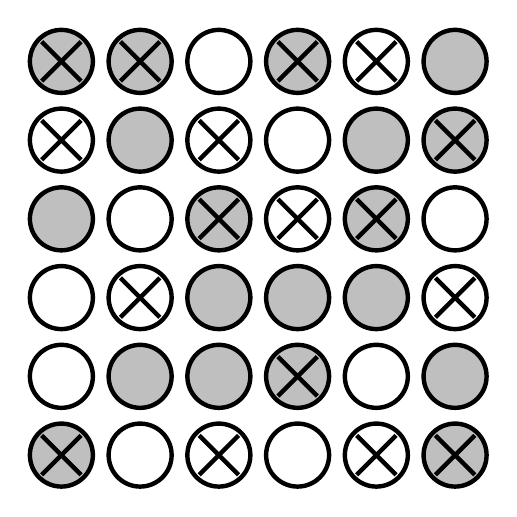
\begin{tikzpicture}
\ExposedSick{0,0}\Person{0,1}\Person{0,2}\Exposed{0,3}\PersonSick{0,4}\ExposedSick{0,5}
\Person{1,0}\Exposed{1,1}\PersonSick{1,2}\Person{1,3}\Exposed{1,4}\ExposedSick{1,5}
\PersonSick{2,0}\Exposed{2,1}\Exposed{2,2}\ExposedSick{2,3}\PersonSick{2,4}\Person{2,5}
\Person{3,0}\ExposedSick{3,1}\Exposed{3,2}\PersonSick{3,3}\Person{3,4}\ExposedSick{3,5}
\PersonSick{4,0}\Person{4,1}\Exposed{4,2}\ExposedSick{4,3}\Exposed{4,4}\PersonSick{4,5}
\ExposedSick{5,0}\Exposed{5,1}\PersonSick{5,2}\Person{5,3}\ExposedSick{5,4}\Exposed{5,5}
\end{tikzpicture}
\\\hline\hline
\end{tabular}

\begin{itemize}
\item Disease A
\begin{MultipleChoice}[itemname=nec-and-suff-a]
\wrong{Necessary but not sufficient}
\wrong{Sufficient but not necessary}
\correct{Necessary and Sufficient}
\wrong{Neither necessary nor sufficient}
\end{MultipleChoice}

\item Disease B
\begin{MultipleChoice}[itemname=nec-and-suff-b]
\wrong{Necessary but not sufficient}
\correct{Sufficient but not necessary}
\wrong{Necessary and Sufficient}
\wrong{Neither necessary nor sufficient}
\end{MultipleChoice}

\item Disease C
\begin{MultipleChoice}[itemname=nec-and-suff-c]
\correct{Necessary but not sufficient}
\wrong{Sufficient but not necessary}
\wrong{Necessary and Sufficient}
\wrong{Neither necessary nor sufficient}
\end{MultipleChoice}

\item Disease D
\begin{MultipleChoice}[itemname=nec-and-suff-d]
\wrong{Necessary but not sufficient}
\wrong{Sufficient but not necessary}
\wrong{Necessary and Sufficient}
\correct{Neither necessary nor sufficient}
\end{MultipleChoice}

\end{itemize}

